\section{Computational Experiments} \label{sec:experiments}
Our goal is to benchmark Optimistic Gittins Indices (OGI) against state-of-the-art algorithms in Bayesian and frequentist setting. Specifically, we compare ourselves against Thomson sampling, Bayes UCB, and IDS. Each of these algorithms has in turn been shown to substantially dominate other extant schemes. We replicate some of the same experiments as in papers of \cite{russo2014learning,kaufmann2012thompson} and then add our own for evaluating the problem with multiple simultaneous arm pulls.  

We consider the OGI algorithm for two values of the look-ahead parameter $K$ ($1$ and $3$) , and in one experiment included for completeness, the case of exact Gittins indices ($K=\infty$). We used a common discount factor schedule in all experiments setting $\gamma_t = 1 - 1/(100 + t)$. The choice of $\alpha = 100$ is second order and our conclusions remain unchanged (and actually appear to improve in an absolute sense) with other choices (we show this in a second set of experiments). 

A major consideration in running the experiments is that the CPU time required to execute IDS (the closest competitor) based on the current suggested implementation is orders of magnitudes greater than that of the index schemes or Thompson Sampling. The main bottleneck is that IDS uses numerical integration,  requiring the calculation of a CDF over, at least, hundreds of iterations. By contrast, the version of OGI with $K=1$ uses 10 iterations of the Newton-Raphson method. In the remainder of this section, we discuss the results.

\subsection{Gaussian}
This experiment (Table~\ref{table:gaussian_experiment1}) replicates one in \cite{russo2014learning}. Here the arms generate Gaussian rewards  $X_{i,t} \sim \mathcal{N}(\theta_i, 1)$ where each $\theta_i$ is independently drawn from a standard Gaussian distribution. We simulate 1000 independent trials with 10 arms and 1000 time periods. The implementation of OGI in this experiment uses $K = 1$. It is difficult to compute exact Gittins indices in this setting, but a classical approximation for Gaussian bandits does exist; see \cite{powell2012optimal}, Chapter 6.1.3. We term the use of that approximation `OGI($\infty$) Approx'.  In addition to regret, we  show the average CPU time taken, in seconds, to execute each trial.
%We also evaluate a policy (labeled `OGI Approx' in the table) that computes a particular closed-form approximation to the Gittins Index given in Chapter 6.1.3 of Powell and Ryzhov \cite{powell2012optimal}. 

\begin{table}[h!]
	\centering
	\begin{tabular}{| c | c | c | c | c | c |} \hline
		\textbf{Algorithm}  & \textbf{OGI(1)} & \textbf{OGI($\infty$) Approx.} & \textbf{IDS} & \textbf{TS} & \textbf{Bayes UCB}\\ \hline
		Mean Regret   & 49.19 & 47.64  &  55.83 & 67.40 & 60.30  \\ \hline
		S.D.  & 51.07 & 50.59 & 65.88 & 47.38 & 45.35 \\ \hline
		1st quartile  & 17.49 & 16.88  & 18.61 & 37.46 & 31.41 \\ \hline
		Median  & 41.72 & 40.99 & 40.79 & 63.06 & 57.71 \\ \hline
		3rd quartile  & 73.24 & 72.26 & 78.76 & 94.52 & 86.40 \\ \hline
		CPU time (s) & 0.02 & 0.01 & 11.18 & 0.01 & 0.02 \\ \hline
	\end{tabular}
	\caption[Table caption text]{Gaussian experiment. OGI(1) denotes OGI with $K =1$, while OGI Approx. uses the approximation to the Gaussian Gittins Index from \cite{powell2012optimal}.}
	\label{table:gaussian_experiment1}
\end{table}

The key feature of the results here is that OGI offers an approximately 10\% improvement in regret over its nearest competitor IDS, and larger improvements (20 and 40 \% respectively) over Bayes UCB and Thompson Sampling. The best performing policy is OGI with the specialized Gaussian approximation since it gives a closer approximation to the Gittins Index. At the same time, OGI is essentially as fast as Thomspon sampling, and three orders of magnitude faster than its nearest competitor (in terms of regret). 


\subsection{Bernoulli}
In this experiment regret is simulated over 1000 periods, with 10 arms each having a uniformly distributed Bernoulli parameter, over 1000 independent trials (Table~\ref{table:bernoulli_experiment1}). We use the same setup as in \cite{russo2014learning} for consistency. 

\begin{table}[h!]
	\centering
	\begin{tabular}{| c| c | c | c | c | c | c | c |} \hline
		\textbf{Algorithm} & \textbf{OGI(1)} & \textbf{OGI(3)} &  \textbf{OGI($\infty$)} & \textbf{IDS} & \textbf{TS} & \textbf{Bayes UCB}  \\ \hline
		Mean Regret &  18.12 & 18.00 & 17.52 & 19.03 & 27.39 & 22.71 \\ \hline
		S.D. & 20.71 & 20.37 &  21.40 & 21.42 & 18.19 & 17.27 \\ \hline
		1st quartile & 6.26 & 5.60 & 4.45 & 5.85 & 14.62 & 10.09 \\ \hline
		Median & 15.08 & 14.84 &12.06 & 14.06 & 23.53 & 18.52 \\ \hline
		3rd quartile & 27.63 & 27.74 & 24.93 & 26.48 & 36.11 & 30.58 \\ \hline
		CPU time (s) & 0.19 & 0.89 & (?) hours & 8.11 & 0.01 & 0.05  \\ \hline
	\end{tabular}
	\caption[Table caption text]{Bernoulli experiment. OGI($K$) denotes the OGI algorithm with a $K$ step approximation and tuning parameter $\alpha = 100$. OGI($\infty$) is the algorithm that uses Gittins Indices.}
	\label{table:bernoulli_experiment1}
\end{table}
Each version of OGI outperforms other algorithms and the one that uses (actual) Gittins Indices has the lowest mean regret. Perhaps, unsurprisingly, when OGI  looks ahead 3 steps it performs marginally better than with a single step. Nevertheless, looking ahead 1 step is a reasonably close approximation to the Gittins Index in the Bernoulli problem. In fact the approximation error, when using an optimistic 1 step approximation, is around 15\% and if $K$ is increased to 3, the error drops to around 4\%.

\begin{figure}[h!]
	\begin{subfigure}{.5\textwidth}
		\centering
		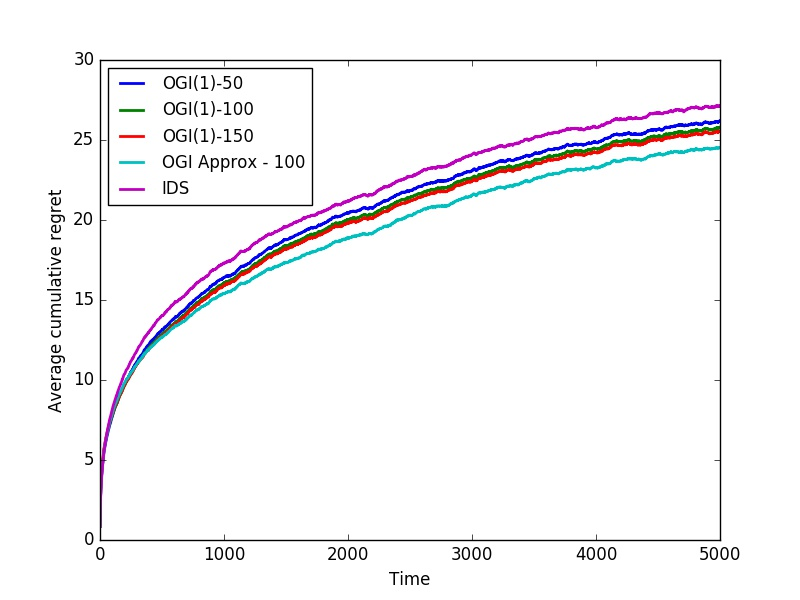
\includegraphics[width=\linewidth]{plots/reduced_gaussian_a.jpg}
		\caption{Gaussian experiment}
		\label{fig:sub1}
	\end{subfigure}
	\begin{subfigure}{.5\textwidth}
		\centering
		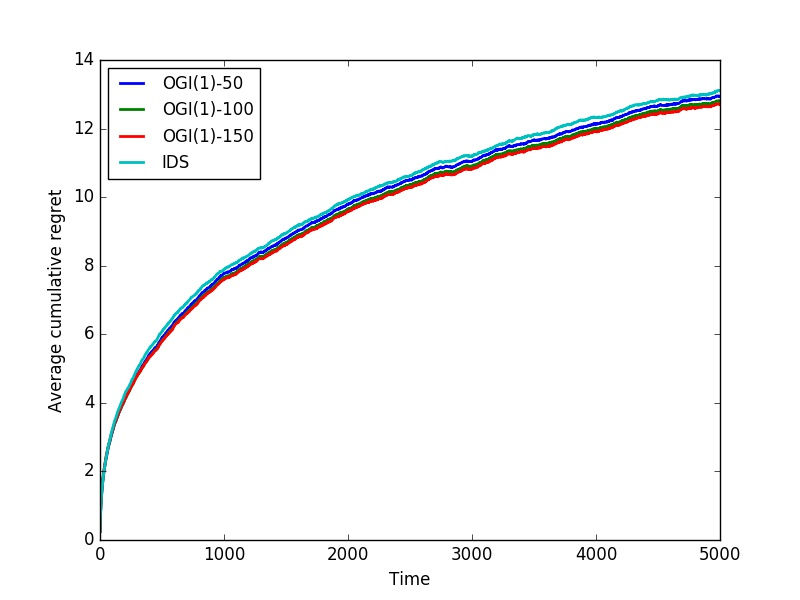
\includegraphics[width=\linewidth]{plots/reduced_figure_a.jpg}
		\caption{Bernoulli experiment}
		\label{fig:sub2}
	\end{subfigure}%
	\caption{Bayesian regret. In the legend, OGI($K$)-$\alpha$ is the format used to indicate parameters $K$ and $\alpha$. The OGI Appox policy uses the approximation to the Gittins index from \cite{powell2012optimal}.}
	\label{fig:bayesian_regret}
\end{figure}
\subsubsection{Longer horizon and robustness}
To understand how Bayes' regret grows in the long run, we simulate Bernoulli and Gaussian bandit problems for a longer horizon of 5000 time steps with the results shown in Figure~\ref{fig:sub1}. 

In the Bernoulli experiment of this section, due to the computational cost, we are only able to simulate OGI with $K = 1$. In addition, to show robustness with respect to the choice of tuning parameter $\alpha$, we show results for $\alpha = 50,100,150$. The message here is essentially the same as in the earlier experiments: the OGI scheme offers a non-trivial performance improvement at a tiny fraction of the computational effort required by its nearest competitor. We omit Thompson Sampling and Bayes UCB from the plots in order to more clearly see the difference between OGI and IDS.

In the Gaussian experiment, we again see that OGI dominates other policies and the tuning parameter has the same effect of lowering regret as it's increased. Also, just as in Table~\ref{table:gaussian_experiment1}, the OGI algorithm that uses the Gaussian-specific approximation has the best performance. 
\subsection{Bayes UCB, \cite{kaufmann2012thompson} experiment} \label{exp:robustness}
For this section that replicates some of the experiments in \cite{kaufmann2012thompson}, we simulate the Bernoulli bandit problem over 500 time steps and with 2 arms. The arms' parameters are fixed to the same values as in \cite{kaufmann2012thompson} and regret is averaged over 5,000 independent trials. We show the results in Figures~\ref{fig:sub3} and ~\ref{fig:sub4}, and as in the Bayes' regret case we see that OGI offers notable performance improvements of Thompson Sampling and Bayes UCB for this modest horizon, but where the arm parameters are fixed rather than being drawn at random.
\begin{figure}[h!]
	\begin{subfigure}{.5\textwidth}
		\centering
		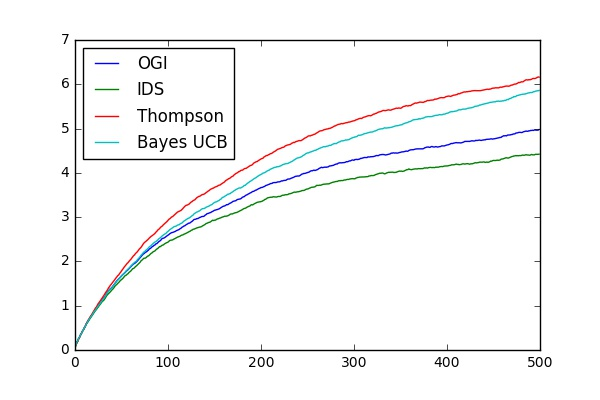
\includegraphics[width=\linewidth]{plots/kaufmann_fig1.jpeg}
		\caption{Bernoulli experiment with two arms and $\mu_1 = 0.1$, $\mu_2 = 0.2$}
		\label{fig:sub3}
	\end{subfigure}
	\begin{subfigure}{.5\textwidth}
		\centering
		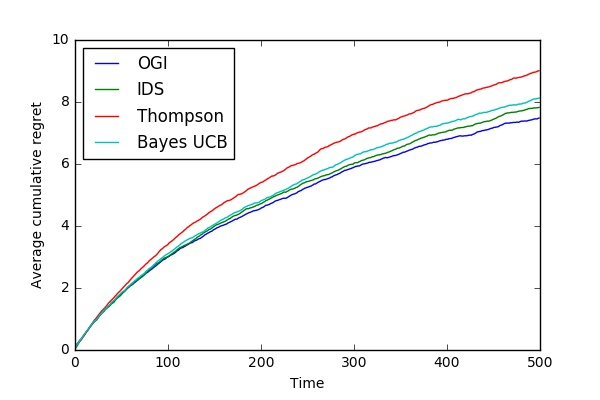
\includegraphics[width=\linewidth]{plots/kaufmann_fig1b.jpeg}
		\caption{Bernoulli experiment with two arms and $\mu_1 = 0.1$, $\mu_2 = 0.2$}
		\label{fig:sub4}
	\end{subfigure}%
	\caption{Frequentist regret. The OGI policy is configured $K=1$ and $\alpha=100$.}
	\label{fig:kaufmann_regret}
\end{figure}

\subsection{Bandits with multiple arm pulls}
We evaluate the heuristics outlined in Section~\ref{sec:multiple_pulls}, for the case when $m$ simultaneous arm pulls are allowed, and compare them against Thompson Sampling and IDS. The implementation of IDS in this setting was the same as for the linear bandits problem; see \citep{russo2014learning} for details. Thompson Sampling was straightforward in that it merely involved sampling from the prior of all arms and picking the arms with the largest $m$ samples. 

For the experiment we have $A = 6$ binary arms with uniformly  distributed biases and fixed $m$ to be 3. We simulate 1000 independent trials and show the results in Figure~\ref{fig:restless1} and Table~\ref{table:restless1_summary}. There is a significant spread in the performance between the OGI-inspired heuristics and both Thompson Sampling and IDS. Again, despite the closest competitor being IDS, the computational cost incurred in running IDS makes Whittle's heuristic, which has the some order of complexity as for the case $m=1$, seem like a particularly attractive algorithm. In fact the implementation of IDS for this experiment required taking Monte-Carlo samples, which can be prohibitively expensive.
\begin{figure}
	\centering
	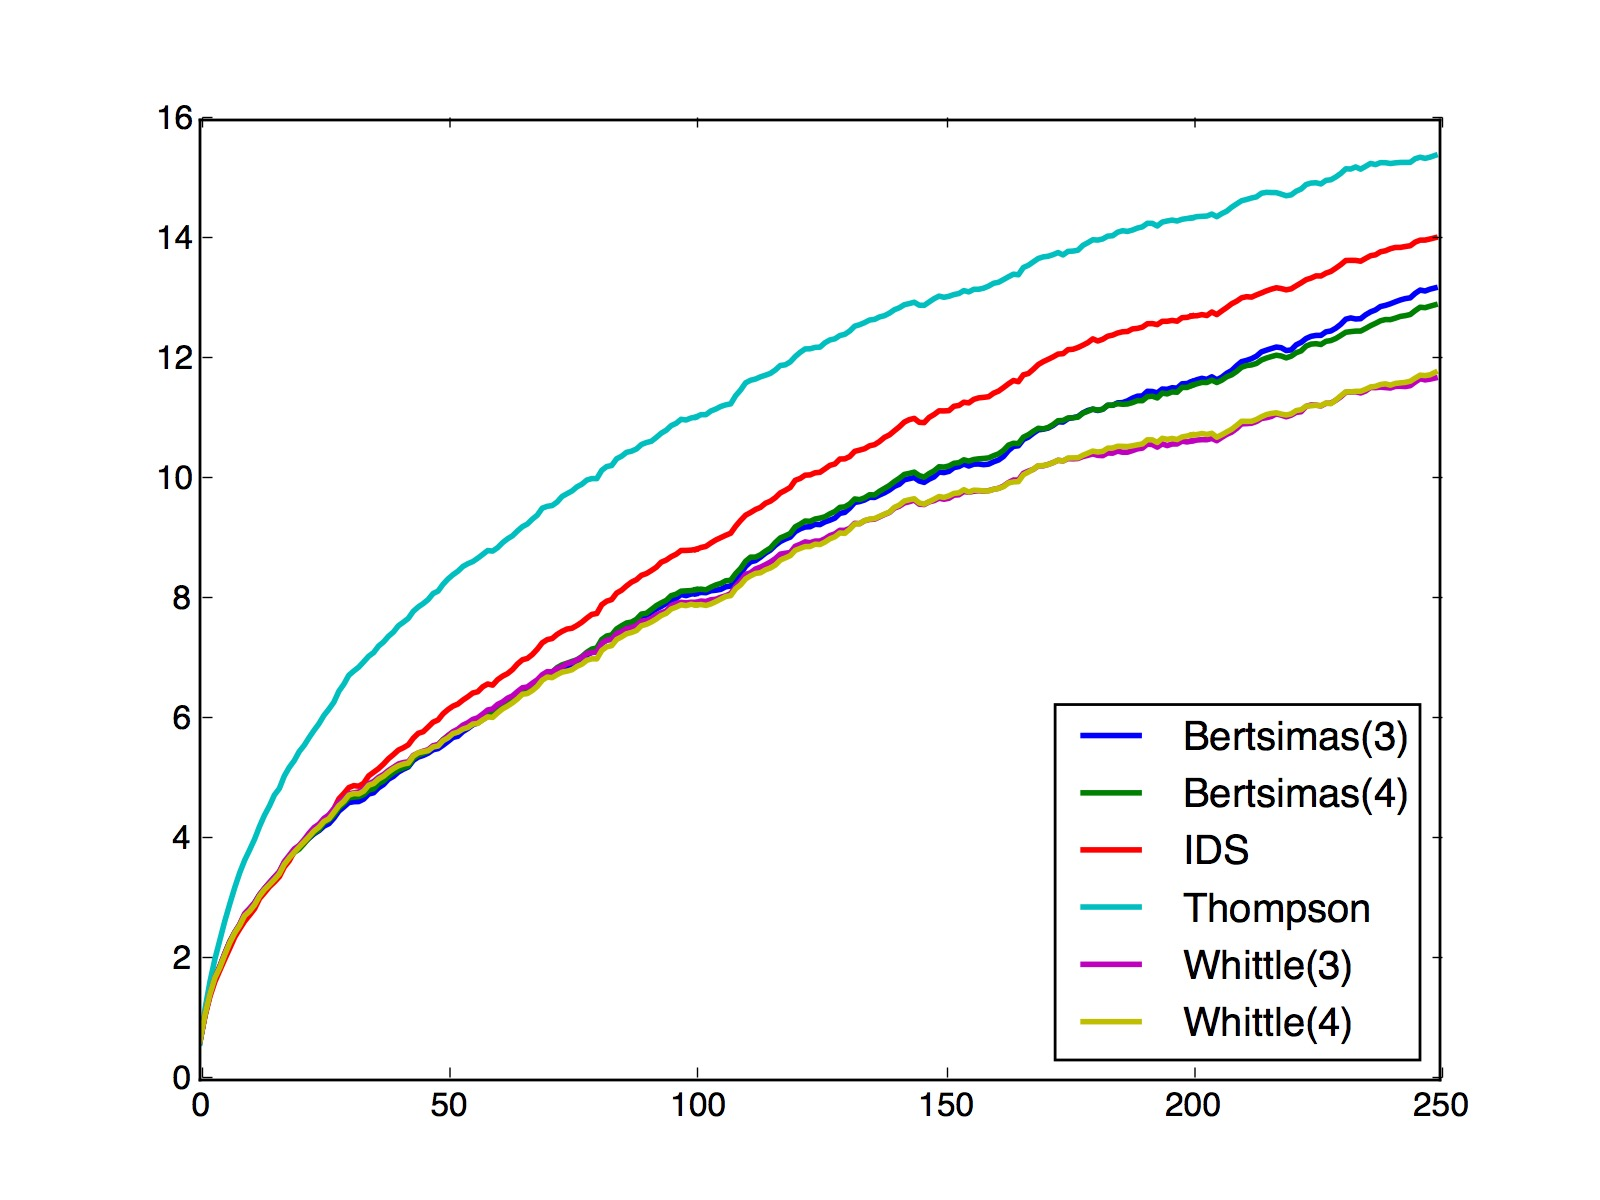
\includegraphics[width=0.5\linewidth]{plots/restless1}
	\caption{Results from restless experiment}
	\label{fig:restless1}
\end{figure}

\begin{table}
	\centering
	\begin{tabular}{lrrrrrr}
		\toprule
		{} &  Bertsimas(3) &  Bertsimas(4) &   IDS &  Thompson &  Whittle(3) &  Whittle(4) \\
		\midrule
		Mean      &         13.20 &         12.92 & 14.04 &     15.41 &       11.70 &       11.79 \\
		Std       &         19.42 &         19.07 & 19.17 &     13.39 &       14.96 &       15.19 \\
		Quartile1 &          0.76 &          0.06 &  1.07 &      6.21 &        1.50 &        1.27 \\
		Median    &         10.06 &          9.87 & 11.21 &     15.08 &       10.68 &       10.56 \\
		Quartile3 &         21.90 &         21.37 & 23.61 &     23.28 &       20.75 &       21.32 \\
		\bottomrule
	\end{tabular}
	\caption{Regret from the multiple arm pulls experiment. ``Whittle($K$)" refers to the Whittle heuristic-like policy described in Section~\ref{sec:multiple_pulls}, using $K$ look-ahead steps. ``Bertsimas($K$)" refers to the alternative heuristic from the same section using the same number of look-ahead steps.}
	\label{table:restless1_summary}
\end{table}